\documentclass[twoside]{book}

% Packages required by doxygen
\usepackage{fixltx2e}
\usepackage{calc}
\usepackage{doxygen}
\usepackage[export]{adjustbox} % also loads graphicx
\usepackage{graphicx}
\usepackage[utf8]{inputenc}
\usepackage{makeidx}
\usepackage{multicol}
\usepackage{multirow}
\PassOptionsToPackage{warn}{textcomp}
\usepackage{textcomp}
\usepackage[nointegrals]{wasysym}
\usepackage[table]{xcolor}

% Font selection
\usepackage[T1]{fontenc}
\usepackage[scaled=.90]{helvet}
\usepackage{courier}
\usepackage{amssymb}
\usepackage{sectsty}
\renewcommand{\familydefault}{\sfdefault}
\allsectionsfont{%
  \fontseries{bc}\selectfont%
  \color{darkgray}%
}
\renewcommand{\DoxyLabelFont}{%
  \fontseries{bc}\selectfont%
  \color{darkgray}%
}
\newcommand{\+}{\discretionary{\mbox{\scriptsize$\hookleftarrow$}}{}{}}

% Page & text layout
\usepackage{geometry}
\geometry{%
  a4paper,%
  top=2.5cm,%
  bottom=2.5cm,%
  left=2.5cm,%
  right=2.5cm%
}
\tolerance=750
\hfuzz=15pt
\hbadness=750
\setlength{\emergencystretch}{15pt}
\setlength{\parindent}{0cm}
\setlength{\parskip}{0.2cm}
\makeatletter
\renewcommand{\paragraph}{%
  \@startsection{paragraph}{4}{0ex}{-1.0ex}{1.0ex}{%
    \normalfont\normalsize\bfseries\SS@parafont%
  }%
}
\renewcommand{\subparagraph}{%
  \@startsection{subparagraph}{5}{0ex}{-1.0ex}{1.0ex}{%
    \normalfont\normalsize\bfseries\SS@subparafont%
  }%
}
\makeatother

% Headers & footers
\usepackage{fancyhdr}
\pagestyle{fancyplain}
\fancyhead[LE]{\fancyplain{}{\bfseries\thepage}}
\fancyhead[CE]{\fancyplain{}{}}
\fancyhead[RE]{\fancyplain{}{\bfseries\leftmark}}
\fancyhead[LO]{\fancyplain{}{\bfseries\rightmark}}
\fancyhead[CO]{\fancyplain{}{}}
\fancyhead[RO]{\fancyplain{}{\bfseries\thepage}}
\fancyfoot[LE]{\fancyplain{}{}}
\fancyfoot[CE]{\fancyplain{}{}}
\fancyfoot[RE]{\fancyplain{}{\bfseries\scriptsize Generated on Fri Jul 17 2015 22\+:05\+:25 for My Project by Doxygen }}
\fancyfoot[LO]{\fancyplain{}{\bfseries\scriptsize Generated on Fri Jul 17 2015 22\+:05\+:25 for My Project by Doxygen }}
\fancyfoot[CO]{\fancyplain{}{}}
\fancyfoot[RO]{\fancyplain{}{}}
\renewcommand{\footrulewidth}{0.4pt}
\renewcommand{\chaptermark}[1]{%
  \markboth{#1}{}%
}
\renewcommand{\sectionmark}[1]{%
  \markright{\thesection\ #1}%
}

% Indices & bibliography
\usepackage{natbib}
\usepackage[titles]{tocloft}
\setcounter{tocdepth}{3}
\setcounter{secnumdepth}{5}
\makeindex

% Hyperlinks (required, but should be loaded last)
\usepackage{ifpdf}
\ifpdf
  \usepackage[pdftex,pagebackref=true]{hyperref}
\else
  \usepackage[ps2pdf,pagebackref=true]{hyperref}
\fi
\hypersetup{%
  colorlinks=true,%
  linkcolor=blue,%
  citecolor=blue,%
  unicode%
}

% Custom commands
\newcommand{\clearemptydoublepage}{%
  \newpage{\pagestyle{empty}\cleardoublepage}%
}


%===== C O N T E N T S =====

\begin{document}

% Titlepage & ToC
\hypersetup{pageanchor=false,
             bookmarks=true,
             bookmarksnumbered=true,
             pdfencoding=unicode
            }
\pagenumbering{roman}
\begin{titlepage}
\vspace*{7cm}
\begin{center}%
{\Large My Project }\\
\vspace*{1cm}
{\large Generated by Doxygen 1.8.9.1}\\
\vspace*{0.5cm}
{\small Fri Jul 17 2015 22:05:25}\\
\end{center}
\end{titlepage}
\clearemptydoublepage
\tableofcontents
\clearemptydoublepage
\pagenumbering{arabic}
\hypersetup{pageanchor=true}

%--- Begin generated contents ---
\chapter{Class Index}
\section{Class List}
Here are the classes, structs, unions and interfaces with brief descriptions\+:\begin{DoxyCompactList}
\item\contentsline{section}{\hyperlink{structGlobalMemory}{Global\+Memory} }{\pageref{structGlobalMemory}}{}
\end{DoxyCompactList}

\chapter{File Index}
\section{File List}
Here is a list of all files with brief descriptions\+:\begin{DoxyCompactList}
\item\contentsline{section}{\hyperlink{fft_8C}{fft.\+C} }{\pageref{fft_8C}}{}
\end{DoxyCompactList}

\chapter{Class Documentation}
\hypertarget{structGlobalMemory}{}\section{Global\+Memory Struct Reference}
\label{structGlobalMemory}\index{Global\+Memory@{Global\+Memory}}
\subsection*{Public Attributes}
\begin{DoxyCompactItemize}
\item 
int \hyperlink{structGlobalMemory_a83c470a5d1c175f7a1acf1b9e3d88f38}{id}
\item 
int $\ast$ \hyperlink{structGlobalMemory_a20ef09094978064a7a728f19746beba0}{transtimes}
\item 
int $\ast$ \hyperlink{structGlobalMemory_a65cad0bb3e74fa2529bf6d05970826e8}{totaltimes}
\item 
int \hyperlink{structGlobalMemory_acdb6d13712d999b9d0ee2699ae8e6742}{starttime}
\item 
int \hyperlink{structGlobalMemory_aea82d496e0ad8bd119115aa20339bde1}{finishtime}
\item 
int \hyperlink{structGlobalMemory_af5a01bd3e84a9eded90836059a8c8265}{initdonetime}
\end{DoxyCompactItemize}


\subsection{Member Data Documentation}
\hypertarget{structGlobalMemory_aea82d496e0ad8bd119115aa20339bde1}{}\index{Global\+Memory@{Global\+Memory}!finishtime@{finishtime}}
\index{finishtime@{finishtime}!Global\+Memory@{Global\+Memory}}
\subsubsection[{finishtime}]{\setlength{\rightskip}{0pt plus 5cm}int Global\+Memory\+::finishtime}\label{structGlobalMemory_aea82d496e0ad8bd119115aa20339bde1}
\hypertarget{structGlobalMemory_a83c470a5d1c175f7a1acf1b9e3d88f38}{}\index{Global\+Memory@{Global\+Memory}!id@{id}}
\index{id@{id}!Global\+Memory@{Global\+Memory}}
\subsubsection[{id}]{\setlength{\rightskip}{0pt plus 5cm}int Global\+Memory\+::id}\label{structGlobalMemory_a83c470a5d1c175f7a1acf1b9e3d88f38}
\hypertarget{structGlobalMemory_af5a01bd3e84a9eded90836059a8c8265}{}\index{Global\+Memory@{Global\+Memory}!initdonetime@{initdonetime}}
\index{initdonetime@{initdonetime}!Global\+Memory@{Global\+Memory}}
\subsubsection[{initdonetime}]{\setlength{\rightskip}{0pt plus 5cm}int Global\+Memory\+::initdonetime}\label{structGlobalMemory_af5a01bd3e84a9eded90836059a8c8265}
\hypertarget{structGlobalMemory_acdb6d13712d999b9d0ee2699ae8e6742}{}\index{Global\+Memory@{Global\+Memory}!starttime@{starttime}}
\index{starttime@{starttime}!Global\+Memory@{Global\+Memory}}
\subsubsection[{starttime}]{\setlength{\rightskip}{0pt plus 5cm}int Global\+Memory\+::starttime}\label{structGlobalMemory_acdb6d13712d999b9d0ee2699ae8e6742}
\hypertarget{structGlobalMemory_a65cad0bb3e74fa2529bf6d05970826e8}{}\index{Global\+Memory@{Global\+Memory}!totaltimes@{totaltimes}}
\index{totaltimes@{totaltimes}!Global\+Memory@{Global\+Memory}}
\subsubsection[{totaltimes}]{\setlength{\rightskip}{0pt plus 5cm}int$\ast$ Global\+Memory\+::totaltimes}\label{structGlobalMemory_a65cad0bb3e74fa2529bf6d05970826e8}
\hypertarget{structGlobalMemory_a20ef09094978064a7a728f19746beba0}{}\index{Global\+Memory@{Global\+Memory}!transtimes@{transtimes}}
\index{transtimes@{transtimes}!Global\+Memory@{Global\+Memory}}
\subsubsection[{transtimes}]{\setlength{\rightskip}{0pt plus 5cm}int$\ast$ Global\+Memory\+::transtimes}\label{structGlobalMemory_a20ef09094978064a7a728f19746beba0}


The documentation for this struct was generated from the following file\+:\begin{DoxyCompactItemize}
\item 
\hyperlink{fft_8C}{fft.\+C}\end{DoxyCompactItemize}

\chapter{File Documentation}
\hypertarget{fft_8C}{}\section{fft.\+C File Reference}
\label{fft_8C}\index{fft.\+C@{fft.\+C}}
{\ttfamily \#include $<$stdio.\+h$>$}\\*
{\ttfamily \#include $<$math.\+h$>$}\\*
Include dependency graph for fft.\+C\+:
\nopagebreak
\begin{figure}[H]
\begin{center}
\leavevmode
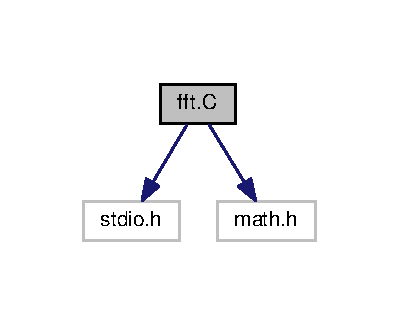
\includegraphics[width=191pt]{fft_8C__incl}
\end{center}
\end{figure}
\subsection*{Classes}
\begin{DoxyCompactItemize}
\item 
struct \hyperlink{structGlobalMemory}{Global\+Memory}
\end{DoxyCompactItemize}
\subsection*{Macros}
\begin{DoxyCompactItemize}
\item 
\#define \hyperlink{fft_8C_a7d467c1d283fdfa1f2081ba1e0d01b6e}{P\+A\+G\+E\+\_\+\+S\+I\+Z\+E}~4096
\item 
\#define \hyperlink{fft_8C_a1cf55e02cd2f0edd18a270fa33314670}{N\+U\+M\+\_\+\+C\+A\+C\+H\+E\+\_\+\+L\+I\+N\+E\+S}~65536
\item 
\#define \hyperlink{fft_8C_a05cb055f4f0f37b23d5697a5af1daa72}{L\+O\+G2\+\_\+\+L\+I\+N\+E\+\_\+\+S\+I\+Z\+E}~4
\item 
\#define \hyperlink{fft_8C_a598a3330b3c21701223ee0ca14316eca}{P\+I}~3.\+1416
\item 
\#define \hyperlink{fft_8C_a383f5d92772af0967bbc18d6cac778a2}{D\+E\+F\+A\+U\+L\+T\+\_\+\+M}~10
\item 
\#define \hyperlink{fft_8C_a5ef8f72e91130f2eaa3a1308437323c3}{D\+E\+F\+A\+U\+L\+T\+\_\+\+P}~1
\item 
\#define \hyperlink{fft_8C_aac9153aee4bdb92701df902e06a74eb3}{S\+W\+A\+P}(a,  b)~\{double tmp; tmp=a; a=b; b=tmp;\}
\end{DoxyCompactItemize}
\subsection*{Functions}
\begin{DoxyCompactItemize}
\item 
void \hyperlink{fft_8C_ae6bcaa881a85c5bc360884a266ba7a48}{Slave\+Start} ()
\item 
double \hyperlink{fft_8C_a05c06b357a7c94983b0b5595ec483d49}{Touch\+Array} (double $\ast$, double $\ast$, double $\ast$, double $\ast$, int, int, int, int)
\item 
void \hyperlink{fft_8C_a288e18636d2be3d008f12b44db70f323}{F\+F\+T1\+D} (int, int, int, double $\ast$, double $\ast$, double $\ast$, double $\ast$, int, int $\ast$, int, int, int, int, int, int, int, struct \hyperlink{structGlobalMemory}{Global\+Memory} $\ast$)
\item 
double \hyperlink{fft_8C_adbf16cb09423a83607a647e9316fb8a3}{Check\+Sum} ()
\item 
double \hyperlink{fft_8C_a0556ac4bd80375e8a98d85ae0f1b4486}{drand48} ()
\item 
int \hyperlink{fft_8C_a89fa0b48e4d41d891cc11bb60c47b811}{log\+\_\+2} (int)
\item 
void \hyperlink{fft_8C_a2297374ee04f814e4f1dde15817d76e0}{printerr} (char $\ast$)
\item 
\hyperlink{fft_8C_a386d026281190375f6ce7c366d48931a}{main} (int argc, char $\ast$argv)
\item 
double \hyperlink{fft_8C_aece45dc7ebe959b213c3e91da5eecefa}{Check\+Sum} (int \hyperlink{fft_8C_a7722c8ecbb62d99aee7ce68b1752f337}{N}, double $\ast$\hyperlink{fft_8C_a711aad4cbe735871dd9e91ab575c878b}{x})
\item 
\hyperlink{fft_8C_ae08491a7b631376d51c872f152d699ed}{Init\+X} (int \hyperlink{fft_8C_a7722c8ecbb62d99aee7ce68b1752f337}{N}, double $\ast$\hyperlink{fft_8C_a711aad4cbe735871dd9e91ab575c878b}{x})
\item 
\hyperlink{fft_8C_ae54c123f4f2c3ce0e7d65f932ba2604b}{Init\+U} (int \hyperlink{fft_8C_a7722c8ecbb62d99aee7ce68b1752f337}{N}, double $\ast$u)
\item 
\hyperlink{fft_8C_aa01c0806ec248364cef3245cb98c055a}{Init\+U2} (int \hyperlink{fft_8C_a7722c8ecbb62d99aee7ce68b1752f337}{N}, double $\ast$u, int n1)
\item 
\hyperlink{fft_8C_ac6a2d1e9a54f1dd85f648c13068c1ad4}{Bit\+Reverse} (int \hyperlink{fft_8C_a5e78dbd5fd0fc01ba7b98dd15e27221e}{M}, int k)
\item 
void \hyperlink{fft_8C_a251fc7139ef1899a1369849ff4b95c0d}{F\+F\+T1\+D} (int direction, int \hyperlink{fft_8C_a5e78dbd5fd0fc01ba7b98dd15e27221e}{M}, int \hyperlink{fft_8C_a7722c8ecbb62d99aee7ce68b1752f337}{N}, double $\ast$\hyperlink{fft_8C_a711aad4cbe735871dd9e91ab575c878b}{x}, double $\ast$scratch, double $\ast$upriv, double $\ast$\hyperlink{fft_8C_ab23232b0d8220f4be701c661c8e8aba7}{umain2}, My\+Num, int $\ast$l\+\_\+transtime, int My\+First, int My\+Last, int \hyperlink{fft_8C_a3d0e20892ce2302560522400f5b5da17}{pad\+\_\+length}, int \hyperlink{fft_8C_aef94be98e2c9e4a4dece75f60ca9792c}{P}, int \hyperlink{fft_8C_a6af31710995648af3fe9c60fbacfd9b0}{test\+\_\+result}, int \hyperlink{fft_8C_a62e849270b0e8c1e2378a94a87858e8b}{doprint}, int \hyperlink{fft_8C_a415f5ce7ea6e1d5f691e8c4d5b2a169f}{dostats}, struct \hyperlink{structGlobalMemory}{Global\+Memory} $\ast$\hyperlink{fft_8C_a6aa784faee19c1ec7661ca843bf221d7}{Global})
\item 
\hyperlink{fft_8C_ab346d9241b82dd3e9a10cee53e1672c5}{Twiddle\+One\+Col} (int direction, int n1, int \hyperlink{fft_8C_a7722c8ecbb62d99aee7ce68b1752f337}{N}, int j, double $\ast$u, double $\ast$\hyperlink{fft_8C_a711aad4cbe735871dd9e91ab575c878b}{x}, int \hyperlink{fft_8C_a3d0e20892ce2302560522400f5b5da17}{pad\+\_\+length})
\item 
\hyperlink{fft_8C_ac37f49e75f15ef2441f5debd361dda7b}{Scale} (int n1, int \hyperlink{fft_8C_a7722c8ecbb62d99aee7ce68b1752f337}{N}, double $\ast$\hyperlink{fft_8C_a711aad4cbe735871dd9e91ab575c878b}{x})
\item 
\hyperlink{fft_8C_aa3fe38d99c028158c9e6656e93e28be9}{Transpose} (int n1, double $\ast$src, double $\ast$dest, int My\+Num, int My\+First, int My\+Last, int \hyperlink{fft_8C_a3d0e20892ce2302560522400f5b5da17}{pad\+\_\+length})
\item 
\hyperlink{fft_8C_afb625e0cb8f22299b2e78c1f3d5662af}{Copy\+Column} (int n1, double $\ast$src, double $\ast$dest)
\item 
\hyperlink{fft_8C_a43a5d3f4a8e26803c9500a9eb70917d1}{Reverse} (int \hyperlink{fft_8C_a7722c8ecbb62d99aee7ce68b1752f337}{N}, int \hyperlink{fft_8C_a5e78dbd5fd0fc01ba7b98dd15e27221e}{M}, double $\ast$\hyperlink{fft_8C_a711aad4cbe735871dd9e91ab575c878b}{x})
\item 
\hyperlink{fft_8C_ab49452f62923f37ebe964d8657bb4bcc}{F\+F\+T1\+D\+Once} (int direction, int \hyperlink{fft_8C_a5e78dbd5fd0fc01ba7b98dd15e27221e}{M}, int \hyperlink{fft_8C_a7722c8ecbb62d99aee7ce68b1752f337}{N}, double $\ast$u, double $\ast$\hyperlink{fft_8C_a711aad4cbe735871dd9e91ab575c878b}{x})
\item 
\hyperlink{fft_8C_a4c95110b84f1e9f2b575122dbf1c1adc}{Print\+Array} (int \hyperlink{fft_8C_a7722c8ecbb62d99aee7ce68b1752f337}{N}, double $\ast$\hyperlink{fft_8C_a711aad4cbe735871dd9e91ab575c878b}{x})
\end{DoxyCompactItemize}
\subsection*{Variables}
\begin{DoxyCompactItemize}
\item 
struct \hyperlink{structGlobalMemory}{Global\+Memory} $\ast$ \hyperlink{fft_8C_a6aa784faee19c1ec7661ca843bf221d7}{Global}
\item 
int \hyperlink{fft_8C_aef94be98e2c9e4a4dece75f60ca9792c}{P} = \hyperlink{fft_8C_a5ef8f72e91130f2eaa3a1308437323c3}{D\+E\+F\+A\+U\+L\+T\+\_\+\+P}
\item 
int \hyperlink{fft_8C_a5e78dbd5fd0fc01ba7b98dd15e27221e}{M} = \hyperlink{fft_8C_a383f5d92772af0967bbc18d6cac778a2}{D\+E\+F\+A\+U\+L\+T\+\_\+\+M}
\item 
int \hyperlink{fft_8C_a7722c8ecbb62d99aee7ce68b1752f337}{N}
\item 
int \hyperlink{fft_8C_a54af42a3fc75a72bd07ecc71cee6f5ba}{root\+N}
\item 
double $\ast$ \hyperlink{fft_8C_a711aad4cbe735871dd9e91ab575c878b}{x}
\item 
double $\ast$ \hyperlink{fft_8C_a261dc6445544ab3a09e5f50b961887b5}{trans}
\item 
double $\ast$ \hyperlink{fft_8C_a482db91d0d238ae4374a2d566ba79efd}{umain}
\item 
double $\ast$ \hyperlink{fft_8C_ab23232b0d8220f4be701c661c8e8aba7}{umain2}
\item 
int \hyperlink{fft_8C_a6af31710995648af3fe9c60fbacfd9b0}{test\+\_\+result} = 0
\item 
int \hyperlink{fft_8C_a62e849270b0e8c1e2378a94a87858e8b}{doprint} = 0
\item 
int \hyperlink{fft_8C_a415f5ce7ea6e1d5f691e8c4d5b2a169f}{dostats} = 0
\item 
int \hyperlink{fft_8C_ac5065349699afaaa137bb3d5176f65a7}{transtime} = 0
\item 
int \hyperlink{fft_8C_ab151086fbe0d880116adb5d5891c6530}{transtime2} = 0
\item 
int \hyperlink{fft_8C_a88a788d7069c5e81d258f34b79a911ef}{avgtranstime} = 0
\item 
int \hyperlink{fft_8C_a65be02baa5bf3f64dc8057a783d6e4c0}{avgcomptime} = 0
\item 
unsigned int \hyperlink{fft_8C_a4b0e5ae3035174e848f5e52f5fd9506f}{transstart} = 0
\item 
unsigned int \hyperlink{fft_8C_a02ddcff0fa450bbe96472988730051ef}{transend} = 0
\item 
int \hyperlink{fft_8C_abaacc1b51e77ad76d3bd569c6a761b50}{maxtotal} =0
\item 
int \hyperlink{fft_8C_ae4ea09b43e337f76159fd601ec785bcf}{mintotal} =0
\item 
double \hyperlink{fft_8C_acff78ed4dd1ec7c0054655fe1ff24e86}{maxfrac} =0
\item 
double \hyperlink{fft_8C_adae7fdc068d0cda31e7c82201018d2cb}{minfrac} =0
\item 
double \hyperlink{fft_8C_a73bf764204b57c2a18707075fac2b429}{avgfractime} =0
\item 
int \hyperlink{fft_8C_ae058fc3d0cfa8f930eb88082726ccf56}{orig\+\_\+num\+\_\+lines} = \hyperlink{fft_8C_a1cf55e02cd2f0edd18a270fa33314670}{N\+U\+M\+\_\+\+C\+A\+C\+H\+E\+\_\+\+L\+I\+N\+E\+S}
\item 
int \hyperlink{fft_8C_aef98a866941663b863e741a502880efc}{num\+\_\+cache\+\_\+lines} = \hyperlink{fft_8C_a1cf55e02cd2f0edd18a270fa33314670}{N\+U\+M\+\_\+\+C\+A\+C\+H\+E\+\_\+\+L\+I\+N\+E\+S}
\item 
int \hyperlink{fft_8C_afdcaa2ef4ede55618f5ff6d5aa53dac6}{log2\+\_\+line\+\_\+size} = \hyperlink{fft_8C_a05cb055f4f0f37b23d5697a5af1daa72}{L\+O\+G2\+\_\+\+L\+I\+N\+E\+\_\+\+S\+I\+Z\+E}
\item 
int \hyperlink{fft_8C_a43a1d2286bbb11edc0c83ec8588dd81d}{line\+\_\+size}
\item 
int \hyperlink{fft_8C_acaaf880fc407fd07db5ee76b758c2078}{rowsperproc}
\item 
double \hyperlink{fft_8C_a29c72e1e55faf8ac079cacc4df9174d9}{ck1}
\item 
double \hyperlink{fft_8C_af5fea8947cca950bbb397c49007717db}{ck3}
\item 
int \hyperlink{fft_8C_a3d0e20892ce2302560522400f5b5da17}{pad\+\_\+length}
\end{DoxyCompactItemize}


\subsection{Macro Definition Documentation}
\hypertarget{fft_8C_a383f5d92772af0967bbc18d6cac778a2}{}\index{fft.\+C@{fft.\+C}!D\+E\+F\+A\+U\+L\+T\+\_\+\+M@{D\+E\+F\+A\+U\+L\+T\+\_\+\+M}}
\index{D\+E\+F\+A\+U\+L\+T\+\_\+\+M@{D\+E\+F\+A\+U\+L\+T\+\_\+\+M}!fft.\+C@{fft.\+C}}
\subsubsection[{D\+E\+F\+A\+U\+L\+T\+\_\+\+M}]{\setlength{\rightskip}{0pt plus 5cm}\#define D\+E\+F\+A\+U\+L\+T\+\_\+\+M~10}\label{fft_8C_a383f5d92772af0967bbc18d6cac778a2}
\hypertarget{fft_8C_a5ef8f72e91130f2eaa3a1308437323c3}{}\index{fft.\+C@{fft.\+C}!D\+E\+F\+A\+U\+L\+T\+\_\+\+P@{D\+E\+F\+A\+U\+L\+T\+\_\+\+P}}
\index{D\+E\+F\+A\+U\+L\+T\+\_\+\+P@{D\+E\+F\+A\+U\+L\+T\+\_\+\+P}!fft.\+C@{fft.\+C}}
\subsubsection[{D\+E\+F\+A\+U\+L\+T\+\_\+\+P}]{\setlength{\rightskip}{0pt plus 5cm}\#define D\+E\+F\+A\+U\+L\+T\+\_\+\+P~1}\label{fft_8C_a5ef8f72e91130f2eaa3a1308437323c3}
\hypertarget{fft_8C_a05cb055f4f0f37b23d5697a5af1daa72}{}\index{fft.\+C@{fft.\+C}!L\+O\+G2\+\_\+\+L\+I\+N\+E\+\_\+\+S\+I\+Z\+E@{L\+O\+G2\+\_\+\+L\+I\+N\+E\+\_\+\+S\+I\+Z\+E}}
\index{L\+O\+G2\+\_\+\+L\+I\+N\+E\+\_\+\+S\+I\+Z\+E@{L\+O\+G2\+\_\+\+L\+I\+N\+E\+\_\+\+S\+I\+Z\+E}!fft.\+C@{fft.\+C}}
\subsubsection[{L\+O\+G2\+\_\+\+L\+I\+N\+E\+\_\+\+S\+I\+Z\+E}]{\setlength{\rightskip}{0pt plus 5cm}\#define L\+O\+G2\+\_\+\+L\+I\+N\+E\+\_\+\+S\+I\+Z\+E~4}\label{fft_8C_a05cb055f4f0f37b23d5697a5af1daa72}
\hypertarget{fft_8C_a1cf55e02cd2f0edd18a270fa33314670}{}\index{fft.\+C@{fft.\+C}!N\+U\+M\+\_\+\+C\+A\+C\+H\+E\+\_\+\+L\+I\+N\+E\+S@{N\+U\+M\+\_\+\+C\+A\+C\+H\+E\+\_\+\+L\+I\+N\+E\+S}}
\index{N\+U\+M\+\_\+\+C\+A\+C\+H\+E\+\_\+\+L\+I\+N\+E\+S@{N\+U\+M\+\_\+\+C\+A\+C\+H\+E\+\_\+\+L\+I\+N\+E\+S}!fft.\+C@{fft.\+C}}
\subsubsection[{N\+U\+M\+\_\+\+C\+A\+C\+H\+E\+\_\+\+L\+I\+N\+E\+S}]{\setlength{\rightskip}{0pt plus 5cm}\#define N\+U\+M\+\_\+\+C\+A\+C\+H\+E\+\_\+\+L\+I\+N\+E\+S~65536}\label{fft_8C_a1cf55e02cd2f0edd18a270fa33314670}
\hypertarget{fft_8C_a7d467c1d283fdfa1f2081ba1e0d01b6e}{}\index{fft.\+C@{fft.\+C}!P\+A\+G\+E\+\_\+\+S\+I\+Z\+E@{P\+A\+G\+E\+\_\+\+S\+I\+Z\+E}}
\index{P\+A\+G\+E\+\_\+\+S\+I\+Z\+E@{P\+A\+G\+E\+\_\+\+S\+I\+Z\+E}!fft.\+C@{fft.\+C}}
\subsubsection[{P\+A\+G\+E\+\_\+\+S\+I\+Z\+E}]{\setlength{\rightskip}{0pt plus 5cm}\#define P\+A\+G\+E\+\_\+\+S\+I\+Z\+E~4096}\label{fft_8C_a7d467c1d283fdfa1f2081ba1e0d01b6e}
\hypertarget{fft_8C_a598a3330b3c21701223ee0ca14316eca}{}\index{fft.\+C@{fft.\+C}!P\+I@{P\+I}}
\index{P\+I@{P\+I}!fft.\+C@{fft.\+C}}
\subsubsection[{P\+I}]{\setlength{\rightskip}{0pt plus 5cm}\#define P\+I~3.\+1416}\label{fft_8C_a598a3330b3c21701223ee0ca14316eca}
\hypertarget{fft_8C_aac9153aee4bdb92701df902e06a74eb3}{}\index{fft.\+C@{fft.\+C}!S\+W\+A\+P@{S\+W\+A\+P}}
\index{S\+W\+A\+P@{S\+W\+A\+P}!fft.\+C@{fft.\+C}}
\subsubsection[{S\+W\+A\+P}]{\setlength{\rightskip}{0pt plus 5cm}\#define S\+W\+A\+P(
\begin{DoxyParamCaption}
\item[{}]{a, }
\item[{}]{b}
\end{DoxyParamCaption}
)~\{double tmp; tmp=a; a=b; b=tmp;\}}\label{fft_8C_aac9153aee4bdb92701df902e06a74eb3}


\subsection{Function Documentation}
\hypertarget{fft_8C_ac6a2d1e9a54f1dd85f648c13068c1ad4}{}\index{fft.\+C@{fft.\+C}!Bit\+Reverse@{Bit\+Reverse}}
\index{Bit\+Reverse@{Bit\+Reverse}!fft.\+C@{fft.\+C}}
\subsubsection[{Bit\+Reverse}]{\setlength{\rightskip}{0pt plus 5cm}Bit\+Reverse (
\begin{DoxyParamCaption}
\item[{int}]{M, }
\item[{int}]{k}
\end{DoxyParamCaption}
)}\label{fft_8C_ac6a2d1e9a54f1dd85f648c13068c1ad4}


Here is the caller graph for this function\+:
\nopagebreak
\begin{figure}[H]
\begin{center}
\leavevmode
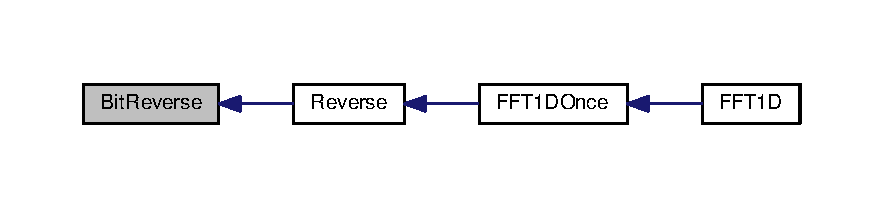
\includegraphics[width=350pt]{fft_8C_ac6a2d1e9a54f1dd85f648c13068c1ad4_icgraph}
\end{center}
\end{figure}


\hypertarget{fft_8C_adbf16cb09423a83607a647e9316fb8a3}{}\index{fft.\+C@{fft.\+C}!Check\+Sum@{Check\+Sum}}
\index{Check\+Sum@{Check\+Sum}!fft.\+C@{fft.\+C}}
\subsubsection[{Check\+Sum}]{\setlength{\rightskip}{0pt plus 5cm}double Check\+Sum (
\begin{DoxyParamCaption}
{}
\end{DoxyParamCaption}
)}\label{fft_8C_adbf16cb09423a83607a647e9316fb8a3}


Here is the caller graph for this function\+:
\nopagebreak
\begin{figure}[H]
\begin{center}
\leavevmode
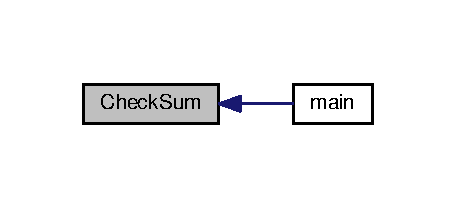
\includegraphics[width=219pt]{fft_8C_adbf16cb09423a83607a647e9316fb8a3_icgraph}
\end{center}
\end{figure}


\hypertarget{fft_8C_aece45dc7ebe959b213c3e91da5eecefa}{}\index{fft.\+C@{fft.\+C}!Check\+Sum@{Check\+Sum}}
\index{Check\+Sum@{Check\+Sum}!fft.\+C@{fft.\+C}}
\subsubsection[{Check\+Sum}]{\setlength{\rightskip}{0pt plus 5cm}double Check\+Sum (
\begin{DoxyParamCaption}
\item[{int}]{N, }
\item[{double $\ast$}]{x}
\end{DoxyParamCaption}
)}\label{fft_8C_aece45dc7ebe959b213c3e91da5eecefa}
\hypertarget{fft_8C_afb625e0cb8f22299b2e78c1f3d5662af}{}\index{fft.\+C@{fft.\+C}!Copy\+Column@{Copy\+Column}}
\index{Copy\+Column@{Copy\+Column}!fft.\+C@{fft.\+C}}
\subsubsection[{Copy\+Column}]{\setlength{\rightskip}{0pt plus 5cm}Copy\+Column (
\begin{DoxyParamCaption}
\item[{int}]{n1, }
\item[{double $\ast$}]{src, }
\item[{double $\ast$}]{dest}
\end{DoxyParamCaption}
)}\label{fft_8C_afb625e0cb8f22299b2e78c1f3d5662af}


Here is the caller graph for this function\+:
\nopagebreak
\begin{figure}[H]
\begin{center}
\leavevmode
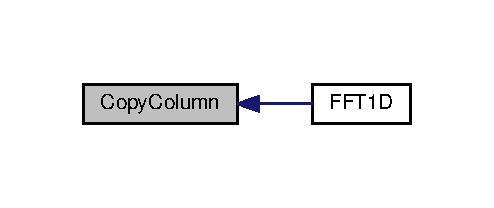
\includegraphics[width=237pt]{fft_8C_afb625e0cb8f22299b2e78c1f3d5662af_icgraph}
\end{center}
\end{figure}


\hypertarget{fft_8C_a0556ac4bd80375e8a98d85ae0f1b4486}{}\index{fft.\+C@{fft.\+C}!drand48@{drand48}}
\index{drand48@{drand48}!fft.\+C@{fft.\+C}}
\subsubsection[{drand48}]{\setlength{\rightskip}{0pt plus 5cm}double drand48 (
\begin{DoxyParamCaption}
{}
\end{DoxyParamCaption}
)}\label{fft_8C_a0556ac4bd80375e8a98d85ae0f1b4486}


Here is the caller graph for this function\+:
\nopagebreak
\begin{figure}[H]
\begin{center}
\leavevmode
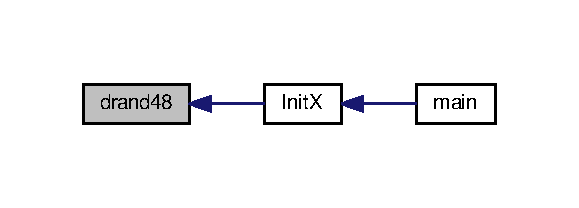
\includegraphics[width=278pt]{fft_8C_a0556ac4bd80375e8a98d85ae0f1b4486_icgraph}
\end{center}
\end{figure}


\hypertarget{fft_8C_a288e18636d2be3d008f12b44db70f323}{}\index{fft.\+C@{fft.\+C}!F\+F\+T1\+D@{F\+F\+T1\+D}}
\index{F\+F\+T1\+D@{F\+F\+T1\+D}!fft.\+C@{fft.\+C}}
\subsubsection[{F\+F\+T1\+D}]{\setlength{\rightskip}{0pt plus 5cm}void F\+F\+T1\+D (
\begin{DoxyParamCaption}
\item[{int}]{, }
\item[{int}]{, }
\item[{int}]{, }
\item[{double $\ast$}]{, }
\item[{double $\ast$}]{, }
\item[{double $\ast$}]{, }
\item[{double $\ast$}]{, }
\item[{int}]{, }
\item[{int $\ast$}]{, }
\item[{int}]{, }
\item[{int}]{, }
\item[{int}]{, }
\item[{int}]{, }
\item[{int}]{, }
\item[{int}]{, }
\item[{int}]{, }
\item[{struct {\bf Global\+Memory} $\ast$}]{}
\end{DoxyParamCaption}
)}\label{fft_8C_a288e18636d2be3d008f12b44db70f323}


Here is the caller graph for this function\+:
\nopagebreak
\begin{figure}[H]
\begin{center}
\leavevmode
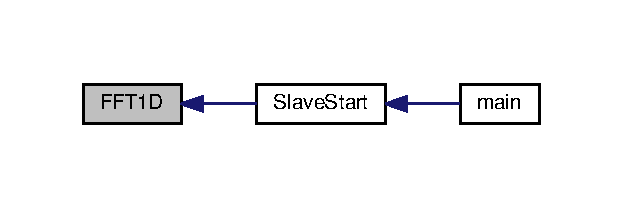
\includegraphics[width=299pt]{fft_8C_a288e18636d2be3d008f12b44db70f323_icgraph}
\end{center}
\end{figure}


\hypertarget{fft_8C_a251fc7139ef1899a1369849ff4b95c0d}{}\index{fft.\+C@{fft.\+C}!F\+F\+T1\+D@{F\+F\+T1\+D}}
\index{F\+F\+T1\+D@{F\+F\+T1\+D}!fft.\+C@{fft.\+C}}
\subsubsection[{F\+F\+T1\+D}]{\setlength{\rightskip}{0pt plus 5cm}void F\+F\+T1\+D (
\begin{DoxyParamCaption}
\item[{int}]{direction, }
\item[{int}]{M, }
\item[{int}]{N, }
\item[{double $\ast$}]{x, }
\item[{double $\ast$}]{scratch, }
\item[{double $\ast$}]{upriv, }
\item[{double $\ast$}]{umain2, }
\item[{My\+Num}]{, }
\item[{int $\ast$}]{l\+\_\+transtime, }
\item[{int}]{My\+First, }
\item[{int}]{My\+Last, }
\item[{int}]{pad\+\_\+length, }
\item[{int}]{P, }
\item[{int}]{test\+\_\+result, }
\item[{int}]{doprint, }
\item[{int}]{dostats, }
\item[{struct {\bf Global\+Memory} $\ast$}]{Global}
\end{DoxyParamCaption}
)}\label{fft_8C_a251fc7139ef1899a1369849ff4b95c0d}


Here is the call graph for this function\+:
\nopagebreak
\begin{figure}[H]
\begin{center}
\leavevmode
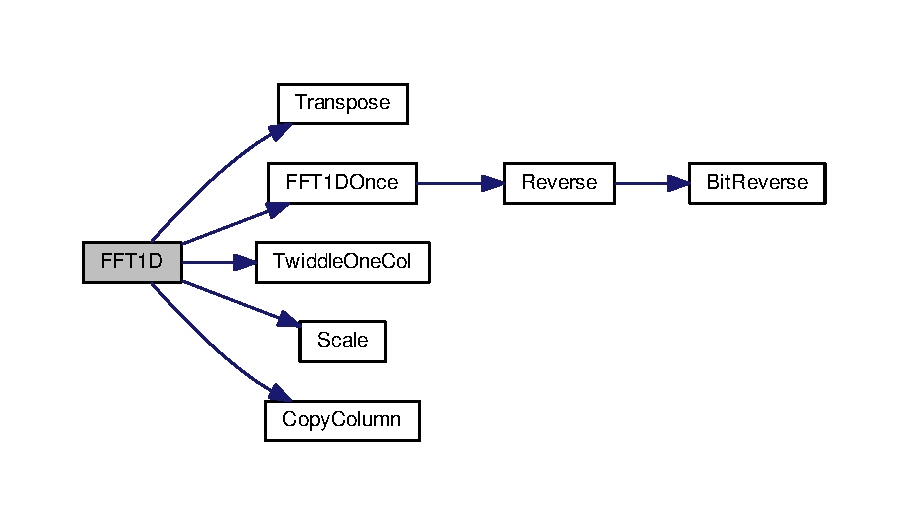
\includegraphics[width=350pt]{fft_8C_a251fc7139ef1899a1369849ff4b95c0d_cgraph}
\end{center}
\end{figure}


\hypertarget{fft_8C_ab49452f62923f37ebe964d8657bb4bcc}{}\index{fft.\+C@{fft.\+C}!F\+F\+T1\+D\+Once@{F\+F\+T1\+D\+Once}}
\index{F\+F\+T1\+D\+Once@{F\+F\+T1\+D\+Once}!fft.\+C@{fft.\+C}}
\subsubsection[{F\+F\+T1\+D\+Once}]{\setlength{\rightskip}{0pt plus 5cm}F\+F\+T1\+D\+Once (
\begin{DoxyParamCaption}
\item[{int}]{direction, }
\item[{int}]{M, }
\item[{int}]{N, }
\item[{double $\ast$}]{u, }
\item[{double $\ast$}]{x}
\end{DoxyParamCaption}
)}\label{fft_8C_ab49452f62923f37ebe964d8657bb4bcc}


Here is the call graph for this function\+:
\nopagebreak
\begin{figure}[H]
\begin{center}
\leavevmode
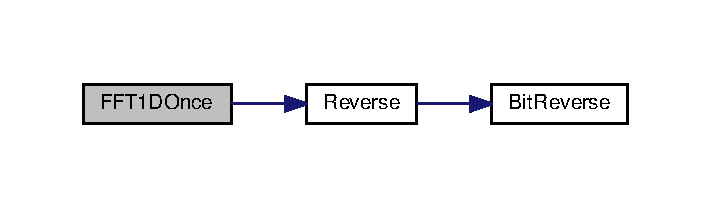
\includegraphics[width=341pt]{fft_8C_ab49452f62923f37ebe964d8657bb4bcc_cgraph}
\end{center}
\end{figure}




Here is the caller graph for this function\+:
\nopagebreak
\begin{figure}[H]
\begin{center}
\leavevmode
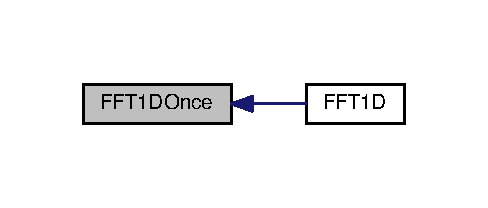
\includegraphics[width=234pt]{fft_8C_ab49452f62923f37ebe964d8657bb4bcc_icgraph}
\end{center}
\end{figure}


\hypertarget{fft_8C_ae54c123f4f2c3ce0e7d65f932ba2604b}{}\index{fft.\+C@{fft.\+C}!Init\+U@{Init\+U}}
\index{Init\+U@{Init\+U}!fft.\+C@{fft.\+C}}
\subsubsection[{Init\+U}]{\setlength{\rightskip}{0pt plus 5cm}Init\+U (
\begin{DoxyParamCaption}
\item[{int}]{N, }
\item[{double $\ast$}]{u}
\end{DoxyParamCaption}
)}\label{fft_8C_ae54c123f4f2c3ce0e7d65f932ba2604b}


Here is the caller graph for this function\+:
\nopagebreak
\begin{figure}[H]
\begin{center}
\leavevmode
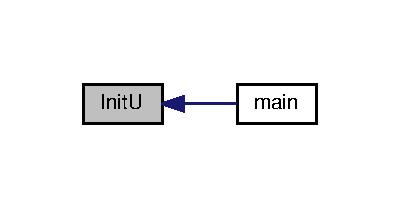
\includegraphics[width=192pt]{fft_8C_ae54c123f4f2c3ce0e7d65f932ba2604b_icgraph}
\end{center}
\end{figure}


\hypertarget{fft_8C_aa01c0806ec248364cef3245cb98c055a}{}\index{fft.\+C@{fft.\+C}!Init\+U2@{Init\+U2}}
\index{Init\+U2@{Init\+U2}!fft.\+C@{fft.\+C}}
\subsubsection[{Init\+U2}]{\setlength{\rightskip}{0pt plus 5cm}Init\+U2 (
\begin{DoxyParamCaption}
\item[{int}]{N, }
\item[{double $\ast$}]{u, }
\item[{int}]{n1}
\end{DoxyParamCaption}
)}\label{fft_8C_aa01c0806ec248364cef3245cb98c055a}


Here is the caller graph for this function\+:
\nopagebreak
\begin{figure}[H]
\begin{center}
\leavevmode
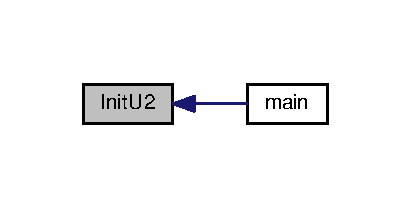
\includegraphics[width=197pt]{fft_8C_aa01c0806ec248364cef3245cb98c055a_icgraph}
\end{center}
\end{figure}


\hypertarget{fft_8C_ae08491a7b631376d51c872f152d699ed}{}\index{fft.\+C@{fft.\+C}!Init\+X@{Init\+X}}
\index{Init\+X@{Init\+X}!fft.\+C@{fft.\+C}}
\subsubsection[{Init\+X}]{\setlength{\rightskip}{0pt plus 5cm}Init\+X (
\begin{DoxyParamCaption}
\item[{int}]{N, }
\item[{double $\ast$}]{x}
\end{DoxyParamCaption}
)}\label{fft_8C_ae08491a7b631376d51c872f152d699ed}


Here is the call graph for this function\+:
\nopagebreak
\begin{figure}[H]
\begin{center}
\leavevmode
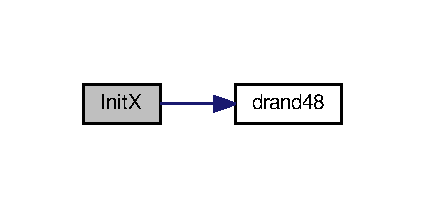
\includegraphics[width=204pt]{fft_8C_ae08491a7b631376d51c872f152d699ed_cgraph}
\end{center}
\end{figure}




Here is the caller graph for this function\+:
\nopagebreak
\begin{figure}[H]
\begin{center}
\leavevmode
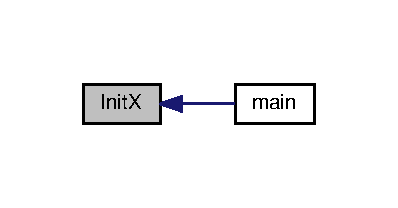
\includegraphics[width=191pt]{fft_8C_ae08491a7b631376d51c872f152d699ed_icgraph}
\end{center}
\end{figure}


\hypertarget{fft_8C_a89fa0b48e4d41d891cc11bb60c47b811}{}\index{fft.\+C@{fft.\+C}!log\+\_\+2@{log\+\_\+2}}
\index{log\+\_\+2@{log\+\_\+2}!fft.\+C@{fft.\+C}}
\subsubsection[{log\+\_\+2}]{\setlength{\rightskip}{0pt plus 5cm}int log\+\_\+2 (
\begin{DoxyParamCaption}
\item[{int}]{number}
\end{DoxyParamCaption}
)}\label{fft_8C_a89fa0b48e4d41d891cc11bb60c47b811}


Here is the caller graph for this function\+:
\nopagebreak
\begin{figure}[H]
\begin{center}
\leavevmode
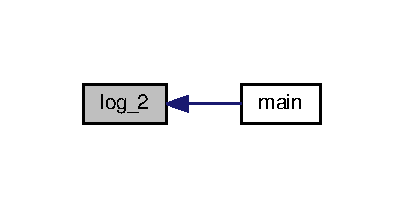
\includegraphics[width=194pt]{fft_8C_a89fa0b48e4d41d891cc11bb60c47b811_icgraph}
\end{center}
\end{figure}


\hypertarget{fft_8C_a386d026281190375f6ce7c366d48931a}{}\index{fft.\+C@{fft.\+C}!main@{main}}
\index{main@{main}!fft.\+C@{fft.\+C}}
\subsubsection[{main}]{\setlength{\rightskip}{0pt plus 5cm}main (
\begin{DoxyParamCaption}
\item[{int}]{argc, }
\item[{char $\ast$}]{argv}
\end{DoxyParamCaption}
)}\label{fft_8C_a386d026281190375f6ce7c366d48931a}


Here is the call graph for this function\+:
\nopagebreak
\begin{figure}[H]
\begin{center}
\leavevmode
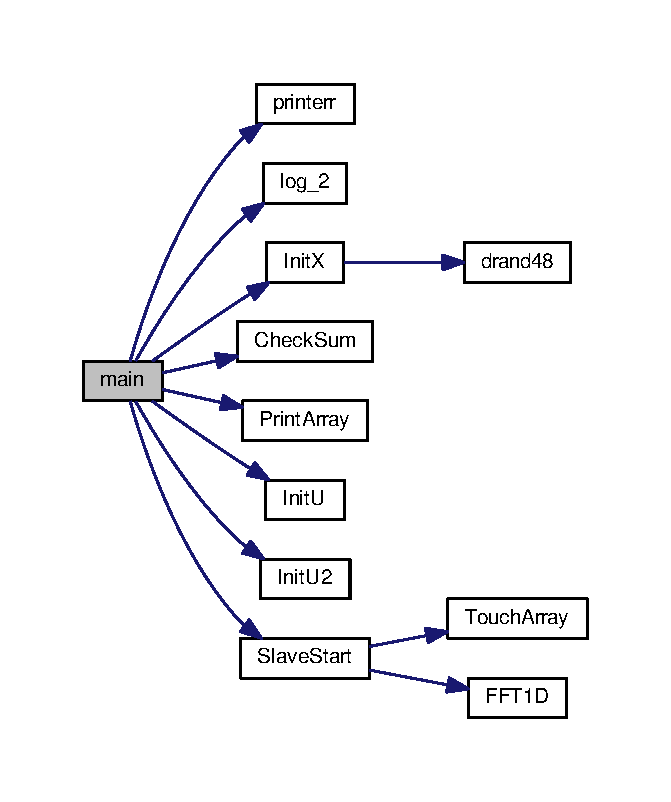
\includegraphics[width=322pt]{fft_8C_a386d026281190375f6ce7c366d48931a_cgraph}
\end{center}
\end{figure}


\hypertarget{fft_8C_a4c95110b84f1e9f2b575122dbf1c1adc}{}\index{fft.\+C@{fft.\+C}!Print\+Array@{Print\+Array}}
\index{Print\+Array@{Print\+Array}!fft.\+C@{fft.\+C}}
\subsubsection[{Print\+Array}]{\setlength{\rightskip}{0pt plus 5cm}Print\+Array (
\begin{DoxyParamCaption}
\item[{int}]{N, }
\item[{double $\ast$}]{x}
\end{DoxyParamCaption}
)}\label{fft_8C_a4c95110b84f1e9f2b575122dbf1c1adc}


Here is the caller graph for this function\+:
\nopagebreak
\begin{figure}[H]
\begin{center}
\leavevmode
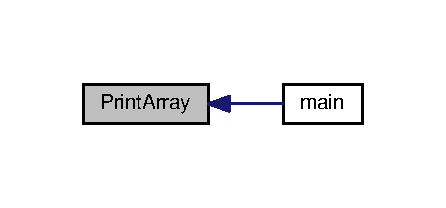
\includegraphics[width=214pt]{fft_8C_a4c95110b84f1e9f2b575122dbf1c1adc_icgraph}
\end{center}
\end{figure}


\hypertarget{fft_8C_a2297374ee04f814e4f1dde15817d76e0}{}\index{fft.\+C@{fft.\+C}!printerr@{printerr}}
\index{printerr@{printerr}!fft.\+C@{fft.\+C}}
\subsubsection[{printerr}]{\setlength{\rightskip}{0pt plus 5cm}void printerr (
\begin{DoxyParamCaption}
\item[{char $\ast$}]{s}
\end{DoxyParamCaption}
)}\label{fft_8C_a2297374ee04f814e4f1dde15817d76e0}


Here is the caller graph for this function\+:
\nopagebreak
\begin{figure}[H]
\begin{center}
\leavevmode
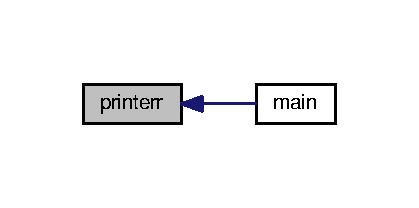
\includegraphics[width=201pt]{fft_8C_a2297374ee04f814e4f1dde15817d76e0_icgraph}
\end{center}
\end{figure}


\hypertarget{fft_8C_a43a5d3f4a8e26803c9500a9eb70917d1}{}\index{fft.\+C@{fft.\+C}!Reverse@{Reverse}}
\index{Reverse@{Reverse}!fft.\+C@{fft.\+C}}
\subsubsection[{Reverse}]{\setlength{\rightskip}{0pt plus 5cm}Reverse (
\begin{DoxyParamCaption}
\item[{int}]{N, }
\item[{int}]{M, }
\item[{double $\ast$}]{x}
\end{DoxyParamCaption}
)}\label{fft_8C_a43a5d3f4a8e26803c9500a9eb70917d1}


Here is the call graph for this function\+:
\nopagebreak
\begin{figure}[H]
\begin{center}
\leavevmode
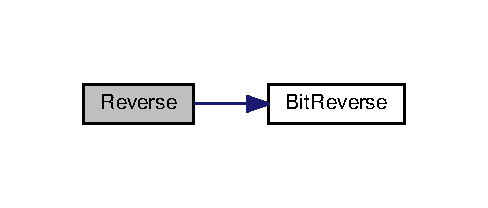
\includegraphics[width=234pt]{fft_8C_a43a5d3f4a8e26803c9500a9eb70917d1_cgraph}
\end{center}
\end{figure}




Here is the caller graph for this function\+:
\nopagebreak
\begin{figure}[H]
\begin{center}
\leavevmode
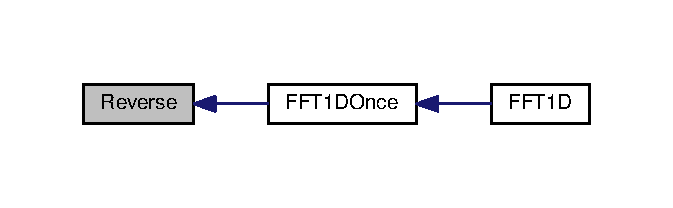
\includegraphics[width=323pt]{fft_8C_a43a5d3f4a8e26803c9500a9eb70917d1_icgraph}
\end{center}
\end{figure}


\hypertarget{fft_8C_ac37f49e75f15ef2441f5debd361dda7b}{}\index{fft.\+C@{fft.\+C}!Scale@{Scale}}
\index{Scale@{Scale}!fft.\+C@{fft.\+C}}
\subsubsection[{Scale}]{\setlength{\rightskip}{0pt plus 5cm}Scale (
\begin{DoxyParamCaption}
\item[{int}]{n1, }
\item[{int}]{N, }
\item[{double $\ast$}]{x}
\end{DoxyParamCaption}
)}\label{fft_8C_ac37f49e75f15ef2441f5debd361dda7b}


Here is the caller graph for this function\+:
\nopagebreak
\begin{figure}[H]
\begin{center}
\leavevmode
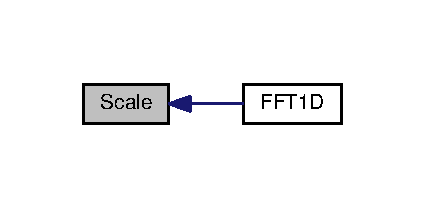
\includegraphics[width=204pt]{fft_8C_ac37f49e75f15ef2441f5debd361dda7b_icgraph}
\end{center}
\end{figure}


\hypertarget{fft_8C_ae6bcaa881a85c5bc360884a266ba7a48}{}\index{fft.\+C@{fft.\+C}!Slave\+Start@{Slave\+Start}}
\index{Slave\+Start@{Slave\+Start}!fft.\+C@{fft.\+C}}
\subsubsection[{Slave\+Start}]{\setlength{\rightskip}{0pt plus 5cm}void Slave\+Start (
\begin{DoxyParamCaption}
{}
\end{DoxyParamCaption}
)}\label{fft_8C_ae6bcaa881a85c5bc360884a266ba7a48}


Here is the call graph for this function\+:
\nopagebreak
\begin{figure}[H]
\begin{center}
\leavevmode
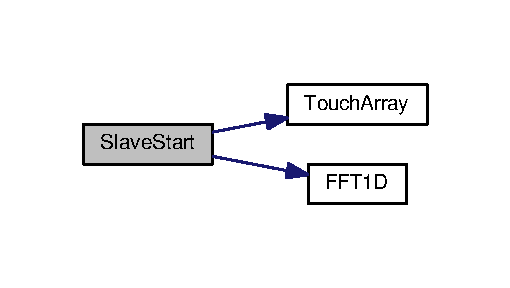
\includegraphics[width=245pt]{fft_8C_ae6bcaa881a85c5bc360884a266ba7a48_cgraph}
\end{center}
\end{figure}




Here is the caller graph for this function\+:
\nopagebreak
\begin{figure}[H]
\begin{center}
\leavevmode
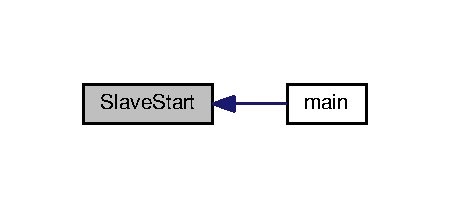
\includegraphics[width=216pt]{fft_8C_ae6bcaa881a85c5bc360884a266ba7a48_icgraph}
\end{center}
\end{figure}


\hypertarget{fft_8C_a05c06b357a7c94983b0b5595ec483d49}{}\index{fft.\+C@{fft.\+C}!Touch\+Array@{Touch\+Array}}
\index{Touch\+Array@{Touch\+Array}!fft.\+C@{fft.\+C}}
\subsubsection[{Touch\+Array}]{\setlength{\rightskip}{0pt plus 5cm}double Touch\+Array (
\begin{DoxyParamCaption}
\item[{double $\ast$}]{x, }
\item[{double $\ast$}]{scratch, }
\item[{double $\ast$}]{u, }
\item[{double $\ast$}]{upriv, }
\item[{int}]{N, }
\item[{int}]{My\+Num, }
\item[{int}]{My\+First, }
\item[{int}]{My\+Last}
\end{DoxyParamCaption}
)}\label{fft_8C_a05c06b357a7c94983b0b5595ec483d49}


Here is the caller graph for this function\+:
\nopagebreak
\begin{figure}[H]
\begin{center}
\leavevmode
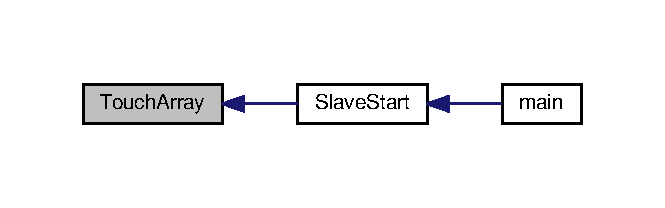
\includegraphics[width=319pt]{fft_8C_a05c06b357a7c94983b0b5595ec483d49_icgraph}
\end{center}
\end{figure}


\hypertarget{fft_8C_aa3fe38d99c028158c9e6656e93e28be9}{}\index{fft.\+C@{fft.\+C}!Transpose@{Transpose}}
\index{Transpose@{Transpose}!fft.\+C@{fft.\+C}}
\subsubsection[{Transpose}]{\setlength{\rightskip}{0pt plus 5cm}Transpose (
\begin{DoxyParamCaption}
\item[{int}]{n1, }
\item[{double $\ast$}]{src, }
\item[{double $\ast$}]{dest, }
\item[{int}]{My\+Num, }
\item[{int}]{My\+First, }
\item[{int}]{My\+Last, }
\item[{int}]{pad\+\_\+length}
\end{DoxyParamCaption}
)}\label{fft_8C_aa3fe38d99c028158c9e6656e93e28be9}


Here is the caller graph for this function\+:
\nopagebreak
\begin{figure}[H]
\begin{center}
\leavevmode
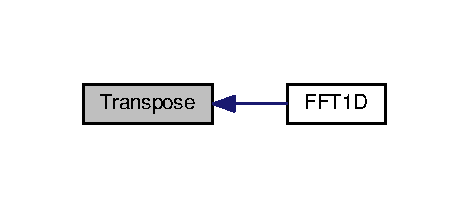
\includegraphics[width=225pt]{fft_8C_aa3fe38d99c028158c9e6656e93e28be9_icgraph}
\end{center}
\end{figure}


\hypertarget{fft_8C_ab346d9241b82dd3e9a10cee53e1672c5}{}\index{fft.\+C@{fft.\+C}!Twiddle\+One\+Col@{Twiddle\+One\+Col}}
\index{Twiddle\+One\+Col@{Twiddle\+One\+Col}!fft.\+C@{fft.\+C}}
\subsubsection[{Twiddle\+One\+Col}]{\setlength{\rightskip}{0pt plus 5cm}Twiddle\+One\+Col (
\begin{DoxyParamCaption}
\item[{int}]{direction, }
\item[{int}]{n1, }
\item[{int}]{N, }
\item[{int}]{j, }
\item[{double $\ast$}]{u, }
\item[{double $\ast$}]{x, }
\item[{int}]{pad\+\_\+length}
\end{DoxyParamCaption}
)}\label{fft_8C_ab346d9241b82dd3e9a10cee53e1672c5}


Here is the caller graph for this function\+:
\nopagebreak
\begin{figure}[H]
\begin{center}
\leavevmode
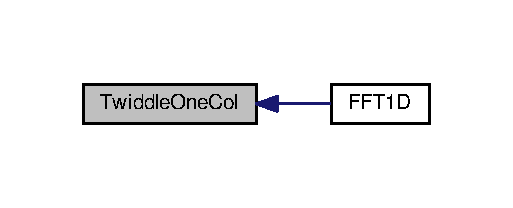
\includegraphics[width=246pt]{fft_8C_ab346d9241b82dd3e9a10cee53e1672c5_icgraph}
\end{center}
\end{figure}




\subsection{Variable Documentation}
\hypertarget{fft_8C_a65be02baa5bf3f64dc8057a783d6e4c0}{}\index{fft.\+C@{fft.\+C}!avgcomptime@{avgcomptime}}
\index{avgcomptime@{avgcomptime}!fft.\+C@{fft.\+C}}
\subsubsection[{avgcomptime}]{\setlength{\rightskip}{0pt plus 5cm}int avgcomptime = 0}\label{fft_8C_a65be02baa5bf3f64dc8057a783d6e4c0}
\hypertarget{fft_8C_a73bf764204b57c2a18707075fac2b429}{}\index{fft.\+C@{fft.\+C}!avgfractime@{avgfractime}}
\index{avgfractime@{avgfractime}!fft.\+C@{fft.\+C}}
\subsubsection[{avgfractime}]{\setlength{\rightskip}{0pt plus 5cm}double avgfractime =0}\label{fft_8C_a73bf764204b57c2a18707075fac2b429}
\hypertarget{fft_8C_a88a788d7069c5e81d258f34b79a911ef}{}\index{fft.\+C@{fft.\+C}!avgtranstime@{avgtranstime}}
\index{avgtranstime@{avgtranstime}!fft.\+C@{fft.\+C}}
\subsubsection[{avgtranstime}]{\setlength{\rightskip}{0pt plus 5cm}int avgtranstime = 0}\label{fft_8C_a88a788d7069c5e81d258f34b79a911ef}
\hypertarget{fft_8C_a29c72e1e55faf8ac079cacc4df9174d9}{}\index{fft.\+C@{fft.\+C}!ck1@{ck1}}
\index{ck1@{ck1}!fft.\+C@{fft.\+C}}
\subsubsection[{ck1}]{\setlength{\rightskip}{0pt plus 5cm}double ck1}\label{fft_8C_a29c72e1e55faf8ac079cacc4df9174d9}
\hypertarget{fft_8C_af5fea8947cca950bbb397c49007717db}{}\index{fft.\+C@{fft.\+C}!ck3@{ck3}}
\index{ck3@{ck3}!fft.\+C@{fft.\+C}}
\subsubsection[{ck3}]{\setlength{\rightskip}{0pt plus 5cm}double ck3}\label{fft_8C_af5fea8947cca950bbb397c49007717db}
\hypertarget{fft_8C_a62e849270b0e8c1e2378a94a87858e8b}{}\index{fft.\+C@{fft.\+C}!doprint@{doprint}}
\index{doprint@{doprint}!fft.\+C@{fft.\+C}}
\subsubsection[{doprint}]{\setlength{\rightskip}{0pt plus 5cm}int doprint = 0}\label{fft_8C_a62e849270b0e8c1e2378a94a87858e8b}
\hypertarget{fft_8C_a415f5ce7ea6e1d5f691e8c4d5b2a169f}{}\index{fft.\+C@{fft.\+C}!dostats@{dostats}}
\index{dostats@{dostats}!fft.\+C@{fft.\+C}}
\subsubsection[{dostats}]{\setlength{\rightskip}{0pt plus 5cm}int dostats = 0}\label{fft_8C_a415f5ce7ea6e1d5f691e8c4d5b2a169f}
\hypertarget{fft_8C_a6aa784faee19c1ec7661ca843bf221d7}{}\index{fft.\+C@{fft.\+C}!Global@{Global}}
\index{Global@{Global}!fft.\+C@{fft.\+C}}
\subsubsection[{Global}]{\setlength{\rightskip}{0pt plus 5cm}struct {\bf Global\+Memory} $\ast$ Global}\label{fft_8C_a6aa784faee19c1ec7661ca843bf221d7}
\hypertarget{fft_8C_a43a1d2286bbb11edc0c83ec8588dd81d}{}\index{fft.\+C@{fft.\+C}!line\+\_\+size@{line\+\_\+size}}
\index{line\+\_\+size@{line\+\_\+size}!fft.\+C@{fft.\+C}}
\subsubsection[{line\+\_\+size}]{\setlength{\rightskip}{0pt plus 5cm}int line\+\_\+size}\label{fft_8C_a43a1d2286bbb11edc0c83ec8588dd81d}
\hypertarget{fft_8C_afdcaa2ef4ede55618f5ff6d5aa53dac6}{}\index{fft.\+C@{fft.\+C}!log2\+\_\+line\+\_\+size@{log2\+\_\+line\+\_\+size}}
\index{log2\+\_\+line\+\_\+size@{log2\+\_\+line\+\_\+size}!fft.\+C@{fft.\+C}}
\subsubsection[{log2\+\_\+line\+\_\+size}]{\setlength{\rightskip}{0pt plus 5cm}int log2\+\_\+line\+\_\+size = {\bf L\+O\+G2\+\_\+\+L\+I\+N\+E\+\_\+\+S\+I\+Z\+E}}\label{fft_8C_afdcaa2ef4ede55618f5ff6d5aa53dac6}
\hypertarget{fft_8C_a5e78dbd5fd0fc01ba7b98dd15e27221e}{}\index{fft.\+C@{fft.\+C}!M@{M}}
\index{M@{M}!fft.\+C@{fft.\+C}}
\subsubsection[{M}]{\setlength{\rightskip}{0pt plus 5cm}int M = {\bf D\+E\+F\+A\+U\+L\+T\+\_\+\+M}}\label{fft_8C_a5e78dbd5fd0fc01ba7b98dd15e27221e}
\hypertarget{fft_8C_acff78ed4dd1ec7c0054655fe1ff24e86}{}\index{fft.\+C@{fft.\+C}!maxfrac@{maxfrac}}
\index{maxfrac@{maxfrac}!fft.\+C@{fft.\+C}}
\subsubsection[{maxfrac}]{\setlength{\rightskip}{0pt plus 5cm}double maxfrac =0}\label{fft_8C_acff78ed4dd1ec7c0054655fe1ff24e86}
\hypertarget{fft_8C_abaacc1b51e77ad76d3bd569c6a761b50}{}\index{fft.\+C@{fft.\+C}!maxtotal@{maxtotal}}
\index{maxtotal@{maxtotal}!fft.\+C@{fft.\+C}}
\subsubsection[{maxtotal}]{\setlength{\rightskip}{0pt plus 5cm}int maxtotal =0}\label{fft_8C_abaacc1b51e77ad76d3bd569c6a761b50}
\hypertarget{fft_8C_adae7fdc068d0cda31e7c82201018d2cb}{}\index{fft.\+C@{fft.\+C}!minfrac@{minfrac}}
\index{minfrac@{minfrac}!fft.\+C@{fft.\+C}}
\subsubsection[{minfrac}]{\setlength{\rightskip}{0pt plus 5cm}double minfrac =0}\label{fft_8C_adae7fdc068d0cda31e7c82201018d2cb}
\hypertarget{fft_8C_ae4ea09b43e337f76159fd601ec785bcf}{}\index{fft.\+C@{fft.\+C}!mintotal@{mintotal}}
\index{mintotal@{mintotal}!fft.\+C@{fft.\+C}}
\subsubsection[{mintotal}]{\setlength{\rightskip}{0pt plus 5cm}int mintotal =0}\label{fft_8C_ae4ea09b43e337f76159fd601ec785bcf}
\hypertarget{fft_8C_a7722c8ecbb62d99aee7ce68b1752f337}{}\index{fft.\+C@{fft.\+C}!N@{N}}
\index{N@{N}!fft.\+C@{fft.\+C}}
\subsubsection[{N}]{\setlength{\rightskip}{0pt plus 5cm}int N}\label{fft_8C_a7722c8ecbb62d99aee7ce68b1752f337}
\hypertarget{fft_8C_aef98a866941663b863e741a502880efc}{}\index{fft.\+C@{fft.\+C}!num\+\_\+cache\+\_\+lines@{num\+\_\+cache\+\_\+lines}}
\index{num\+\_\+cache\+\_\+lines@{num\+\_\+cache\+\_\+lines}!fft.\+C@{fft.\+C}}
\subsubsection[{num\+\_\+cache\+\_\+lines}]{\setlength{\rightskip}{0pt plus 5cm}int num\+\_\+cache\+\_\+lines = {\bf N\+U\+M\+\_\+\+C\+A\+C\+H\+E\+\_\+\+L\+I\+N\+E\+S}}\label{fft_8C_aef98a866941663b863e741a502880efc}
\hypertarget{fft_8C_ae058fc3d0cfa8f930eb88082726ccf56}{}\index{fft.\+C@{fft.\+C}!orig\+\_\+num\+\_\+lines@{orig\+\_\+num\+\_\+lines}}
\index{orig\+\_\+num\+\_\+lines@{orig\+\_\+num\+\_\+lines}!fft.\+C@{fft.\+C}}
\subsubsection[{orig\+\_\+num\+\_\+lines}]{\setlength{\rightskip}{0pt plus 5cm}int orig\+\_\+num\+\_\+lines = {\bf N\+U\+M\+\_\+\+C\+A\+C\+H\+E\+\_\+\+L\+I\+N\+E\+S}}\label{fft_8C_ae058fc3d0cfa8f930eb88082726ccf56}
\hypertarget{fft_8C_aef94be98e2c9e4a4dece75f60ca9792c}{}\index{fft.\+C@{fft.\+C}!P@{P}}
\index{P@{P}!fft.\+C@{fft.\+C}}
\subsubsection[{P}]{\setlength{\rightskip}{0pt plus 5cm}int P = {\bf D\+E\+F\+A\+U\+L\+T\+\_\+\+P}}\label{fft_8C_aef94be98e2c9e4a4dece75f60ca9792c}
\hypertarget{fft_8C_a3d0e20892ce2302560522400f5b5da17}{}\index{fft.\+C@{fft.\+C}!pad\+\_\+length@{pad\+\_\+length}}
\index{pad\+\_\+length@{pad\+\_\+length}!fft.\+C@{fft.\+C}}
\subsubsection[{pad\+\_\+length}]{\setlength{\rightskip}{0pt plus 5cm}int pad\+\_\+length}\label{fft_8C_a3d0e20892ce2302560522400f5b5da17}
\hypertarget{fft_8C_a54af42a3fc75a72bd07ecc71cee6f5ba}{}\index{fft.\+C@{fft.\+C}!root\+N@{root\+N}}
\index{root\+N@{root\+N}!fft.\+C@{fft.\+C}}
\subsubsection[{root\+N}]{\setlength{\rightskip}{0pt plus 5cm}int root\+N}\label{fft_8C_a54af42a3fc75a72bd07ecc71cee6f5ba}
\hypertarget{fft_8C_acaaf880fc407fd07db5ee76b758c2078}{}\index{fft.\+C@{fft.\+C}!rowsperproc@{rowsperproc}}
\index{rowsperproc@{rowsperproc}!fft.\+C@{fft.\+C}}
\subsubsection[{rowsperproc}]{\setlength{\rightskip}{0pt plus 5cm}int rowsperproc}\label{fft_8C_acaaf880fc407fd07db5ee76b758c2078}
\hypertarget{fft_8C_a6af31710995648af3fe9c60fbacfd9b0}{}\index{fft.\+C@{fft.\+C}!test\+\_\+result@{test\+\_\+result}}
\index{test\+\_\+result@{test\+\_\+result}!fft.\+C@{fft.\+C}}
\subsubsection[{test\+\_\+result}]{\setlength{\rightskip}{0pt plus 5cm}int test\+\_\+result = 0}\label{fft_8C_a6af31710995648af3fe9c60fbacfd9b0}
\hypertarget{fft_8C_a261dc6445544ab3a09e5f50b961887b5}{}\index{fft.\+C@{fft.\+C}!trans@{trans}}
\index{trans@{trans}!fft.\+C@{fft.\+C}}
\subsubsection[{trans}]{\setlength{\rightskip}{0pt plus 5cm}double$\ast$ trans}\label{fft_8C_a261dc6445544ab3a09e5f50b961887b5}
\hypertarget{fft_8C_a02ddcff0fa450bbe96472988730051ef}{}\index{fft.\+C@{fft.\+C}!transend@{transend}}
\index{transend@{transend}!fft.\+C@{fft.\+C}}
\subsubsection[{transend}]{\setlength{\rightskip}{0pt plus 5cm}unsigned int transend = 0}\label{fft_8C_a02ddcff0fa450bbe96472988730051ef}
\hypertarget{fft_8C_a4b0e5ae3035174e848f5e52f5fd9506f}{}\index{fft.\+C@{fft.\+C}!transstart@{transstart}}
\index{transstart@{transstart}!fft.\+C@{fft.\+C}}
\subsubsection[{transstart}]{\setlength{\rightskip}{0pt plus 5cm}unsigned int transstart = 0}\label{fft_8C_a4b0e5ae3035174e848f5e52f5fd9506f}
\hypertarget{fft_8C_ac5065349699afaaa137bb3d5176f65a7}{}\index{fft.\+C@{fft.\+C}!transtime@{transtime}}
\index{transtime@{transtime}!fft.\+C@{fft.\+C}}
\subsubsection[{transtime}]{\setlength{\rightskip}{0pt plus 5cm}int transtime = 0}\label{fft_8C_ac5065349699afaaa137bb3d5176f65a7}
\hypertarget{fft_8C_ab151086fbe0d880116adb5d5891c6530}{}\index{fft.\+C@{fft.\+C}!transtime2@{transtime2}}
\index{transtime2@{transtime2}!fft.\+C@{fft.\+C}}
\subsubsection[{transtime2}]{\setlength{\rightskip}{0pt plus 5cm}int transtime2 = 0}\label{fft_8C_ab151086fbe0d880116adb5d5891c6530}
\hypertarget{fft_8C_a482db91d0d238ae4374a2d566ba79efd}{}\index{fft.\+C@{fft.\+C}!umain@{umain}}
\index{umain@{umain}!fft.\+C@{fft.\+C}}
\subsubsection[{umain}]{\setlength{\rightskip}{0pt plus 5cm}double$\ast$ umain}\label{fft_8C_a482db91d0d238ae4374a2d566ba79efd}
\hypertarget{fft_8C_ab23232b0d8220f4be701c661c8e8aba7}{}\index{fft.\+C@{fft.\+C}!umain2@{umain2}}
\index{umain2@{umain2}!fft.\+C@{fft.\+C}}
\subsubsection[{umain2}]{\setlength{\rightskip}{0pt plus 5cm}double$\ast$ umain2}\label{fft_8C_ab23232b0d8220f4be701c661c8e8aba7}
\hypertarget{fft_8C_a711aad4cbe735871dd9e91ab575c878b}{}\index{fft.\+C@{fft.\+C}!x@{x}}
\index{x@{x}!fft.\+C@{fft.\+C}}
\subsubsection[{x}]{\setlength{\rightskip}{0pt plus 5cm}double$\ast$ x}\label{fft_8C_a711aad4cbe735871dd9e91ab575c878b}

%--- End generated contents ---

% Index
\backmatter
\newpage
\phantomsection
\clearemptydoublepage
\addcontentsline{toc}{chapter}{Index}
\printindex

\end{document}
